

\chapter { Etude préliminaire du projet }


\section*{Introduction}
\addcontentsline{toc}{section}{Introduction}
\bigskip
Dans le cadre de la mise en place d'une application de gestion des parking des entreprises, il est essentiel de réaliser une étude préalable approfondie afin de cerner les besoins, les contraintes et les objectifs liés à ce projet. Cette étude préalable permettra de définir les contours du projet et de poser les bases pour son développement et sa mise en œuvre.
Nous commençons par placer le projet dans son cadre général et d'exposer le contexte de travail ainsi que  les objectifs a atteindre.

%_________________________________________________________________________________________________

\section{Présentation de l’organisme d’accueil}
\bigskip
Digital Identity, connue sous l’abréviation « DIGID »est une entreprise tunisienne Fondée en 2019, spécialisée dans le conseil et le développement de solutions technologiques spécifiques à l'échelle nationale et internationale. Ses objectifs sont de permettre à ses clients de se concentrer sur leurs activités principales, en s'appuyant sur des solutions fiables et sur un partenaire crédible et inébranlable.\\
\newline DIGID est spécialisée dans le conseil et la mise en œuvre de solutions logicielles de gestion intégrée.

\bigskip
\begin{figure}[ht]
    \centering
    
\includegraphics[scale = 0.5]{chap1.images/digidlogo.png}
    \caption{Logo de l’entreprise « DIGITAL IDENTITY »}
    \label{Logo de l’entreprise « DIGITAL IDENTITY » }
\end{figure}

%____________


\newpage
\subsection{ Organigramme de l’entreprise }

L’organigramme de Digital Identity figure 1.2 présente une vue parfaite de l’oraganisation des
liens hiéarchiques entre les différentes équipes. En effet, c’est une traduction schématique des
objectifs, des missions et des relations fonctionnelles.

\begin{figure}[ht]
    \centering
    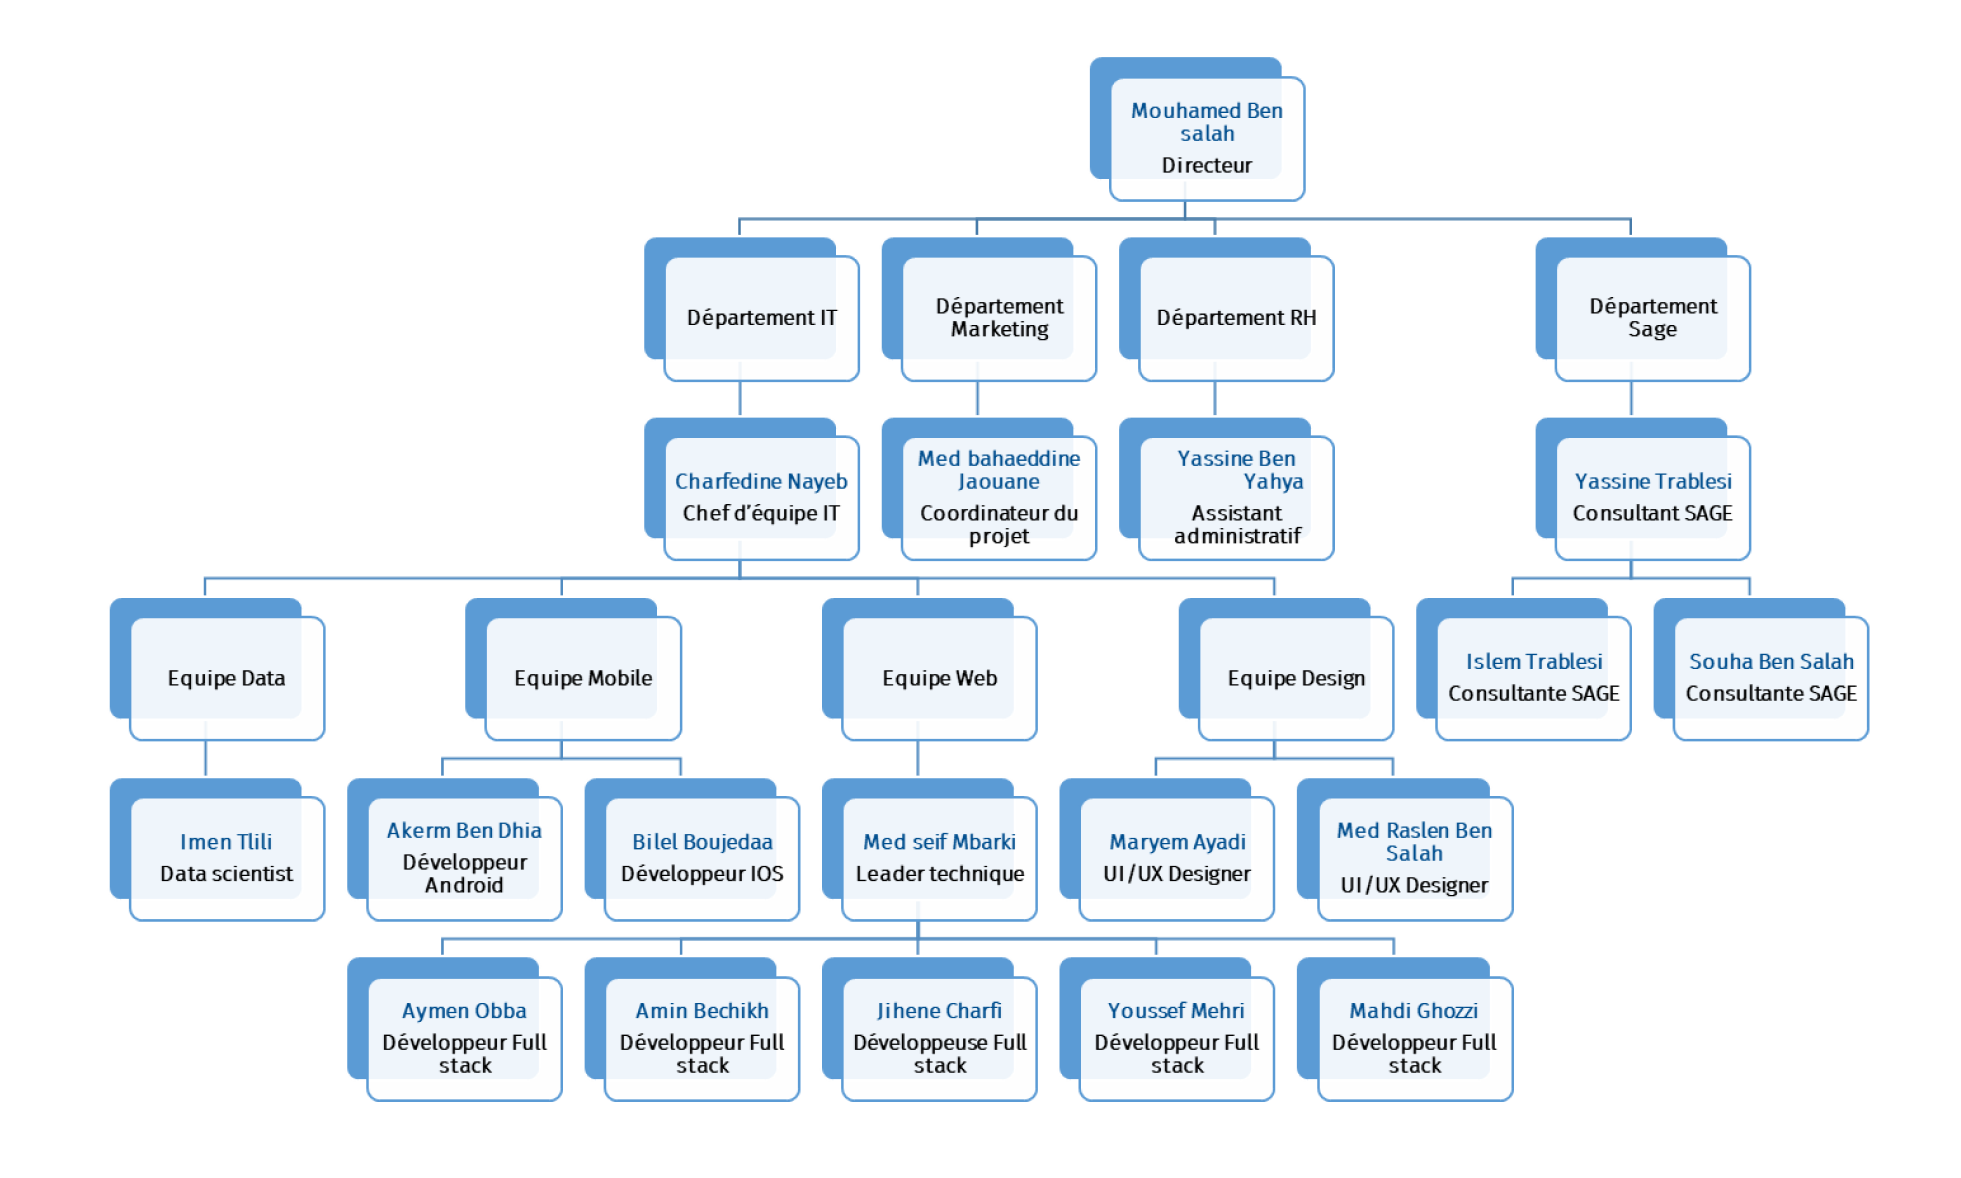
\includegraphics[width=1.1\textwidth,height=12.5cm]{chap1.images/org digid.png}
    \caption{Organigramme de Digital identity}
    \label{fig:orgcogecom}
\end{figure}


\subsection{ Les activités de Digital Identity  }
\begin{figure}[ht]
    \centering
    \includegraphics[width=1\textwidth,height=4.1cm]{chap1.images/digid activités.png}
    \caption{Les activités de Digital Identity}
\end{figure}
\newpage
\textbf{Digital Identity se spécialise dans plusieurs domaines clés :}\\
\begin{itemize}

    \item[$\bullet$] \textbf {Audit et Conseils :} Spécialisée dans les services d'audit et de conseil de haute qualité, Digital Identity aide les entreprises à relever des défis complexes et à atteindre leurs objectifs grâce à une expertise approfondie et une approche personnalisée. Ses recommandations stratégiques optimisent les performances et favorisent une croissance durable.\\

    \item[$\bullet$] \textbf {Implémentation de Systèmes d'Informations :} En tant que fournisseur de confiance, Digital Identity facilite l'adoption de solutions logicielles robustes, garantissant une intégration fluide, une mise en œuvre efficace et une formation complète pour rationaliser les opérations des entreprises et optimiser leur productivité.\\

    \item[$\bullet$] \textbf {Développement d'Applications :} Digital Identity excelle dans le développement d'applications de bureau et mobiles sur mesure, mettant l'accent sur la convivialité et l'utilisation des technologies avancées. Ses solutions personnalisées permettent aux organisations d'optimiser leurs flux de travail de manière transparente.\\

    \item[$\bullet$] \textbf {Infrastructure des Technologies de l'Information :} Elle propose des services complets pour assurer des environnements informatiques fiables, sécurisés et évolutifs, en se spécialisant dans l'architecture réseau, l'intégration de systèmes et la cybersécurité pour garantir des performances optimales.\\

\end{itemize}


\section{Cadre du projet}
\bigskip
Dans cette section, nous allons aborder en détail la problématique soulevée et nous allons présenter une solution pertinente qui a été proposée pour y remédier.
\bigskip
\subsection{ Problématique}
\bigskip
Dans le contexte actuel, la gestion des parcs de véhicules d’entreprise est confrontée à plusieurs défis critiques. La diversité des véhicules et des itinéraires, combinée aux exigences opérationnelles spécifiques de chaque entreprise, rend la gestion des flottes complexe et nécessite des solutions personnalisées. Les entreprises doivent également faire face à des pressions technologiques, telles que l’intégration de nouvelles technologies de suivi et de maintenance prédictive, ainsi qu'à des pratiques durables.\\

Pour répondre à ces défis, une plateforme intégrée capable de fournir une surveillance en temps réel et des analyses prédictives est essentielle. Une telle plateforme doit permettre une optimisation avancée des ressources, en minimisant les coûts et en maximisant l’efficacité opérationnelle. De plus, elle doit intégrer des fonctionnalités de sécurité et de conformité réglementaire pour assurer des opérations sécurisées et conformes aux exigences légales.



%_________________________________________________________________________________________________

\subsection{ Solution proposée}
\bigskip
Notre solution propose une plateforme de gestion de flotte de véhicules d’entreprise qui intègre des technologies avancées pour offrir des fonctionnalités complètes et personnalisables. Cette plateforme permet de surveiller les performances de la flotte en temps réel, de prédire les besoins de maintenance et d’optimiser les itinéraires et l’utilisation des véhicules. Elle offre une gestion centralisée et simplifiée des actifs de transport, réduisant ainsi les coûts opérationnels et augmentant l’efficacité.\\

La dimension Business Intelligence (BI) de la plateforme permet d’analyser les données de manière approfondie, fournissant aux gestionnaires des informations stratégiques essentielles pour la prise de décision. Les tableaux de bord interactifs offrent une vue d’ensemble en temps réel des performances de la flotte, permettant aux gestionnaires de suivre des indicateurs clés tels que le taux d’utilisation des véhicules, les coûts de maintenance et les temps d’immobilisation. Les rapports personnalisables fournissent des insights détaillés sur les tendances et les opportunités d’optimisation, facilitant ainsi une gestion proactive et informée.\\

En intégrant ces fonctionnalités avec une approche centrée sur les besoins des entreprises, notre solution vise à optimiser la gestion des flottes de véhicules, réduisant les coûts et améliorant l’efficacité opérationnelle. Elle permet aux entreprises de rester compétitives en offrant une gestion stratégique et évolutive de leurs actifs de transport, capable de s’adapter aux défis futurs grâce à des technologies émergentes telles que l’intelligence artificielle et l’Internet des objets (IoT).\\


%______________________________________________________________________________________________


\section{Méthodologie et langage de conception}
La conception est cruciale dans le développement d'un système informatique pour répondre aux besoins du client. Les choix conceptuels concernant l'approche, le langage de modélisation et le processus de développement sont issus de réflexions collectives. Nous avons choisi la méthodologie Scrum, une méthode agile, pour réaliser notre projet.
\subsection { Méthodes agiles}
\noindent Parmi les méthodes agiles les plus couramment utilisées de nos jours, on peut citer :

\begin{itemize}[label=$\square$]
    \item Extrême Programming (XP)
    \item Scrum
    \item Agile Unified Process (Agile UP ou AUP)
\end{itemize}


Ces approche agile se caractérise par une méthode itérative et incrémentale, une focalisation sur les besoins des utilisateurs, une flexibilité pour s'adapter aux changements, une collaboration étroite avec toutes les parties prenantes du projet, et une livraison régulière de fonctionnalités à forte valeur ajoutée. Chaque méthode agile présente ses propres pratiques, rôles, cérémonies et outils, tout en partageant les mêmes valeurs et principes fondamentaux de l'agilité.\\

Dans notre contexte, nous avons opté pour le framework Scrum pour le développement de notre application, car il nous semble le mieux adapté à notre travail. Scrum offre une structure agile et flexible qui nous permet de diviser notre projet en sprints. Cette approche itérative nous aide à gérer efficacement notre travail en nous concentrant sur des objectifs clairs à atteindre à chaque étape du développement.


%_________________________________________________________________________________________________



\subsection{ Principes du framework Scrum}
Scrum est un cadre de travail pour la gestion de projet agile qui est largement utilisé à travers le monde. Il comprend des rôles bien définis, un rythme itératif, des réunions chronométrées et des artefacts tels que le product backlog, le sprint backlog et le graphique d'avancement (Burndown Chart). Ces éléments constituent les piliers du processus de gestion de projet agile offert par Scrum.\\

\begin{figure}[htbp]
    \centering
    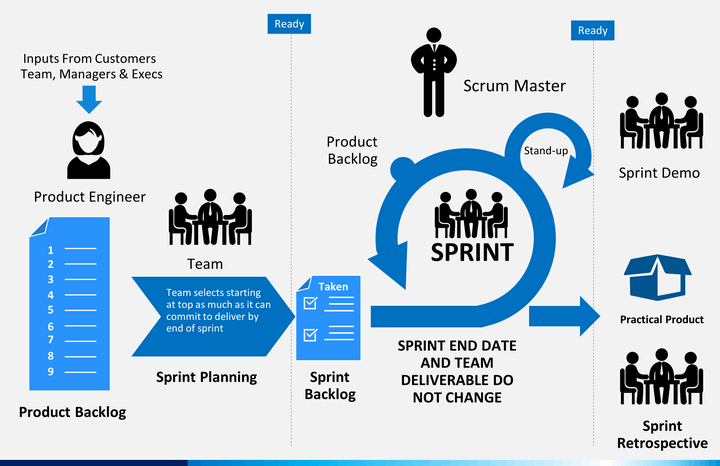
\includegraphics[width=0.9\textwidth,height=9cm]{chap1.images/scrum-process-slide2_2.png}
    \caption{Mode de fonctionnement de la méthodologie Scrum}\cite{ref1}
\end{figure}



\noindent\textbf{Sprint} : Tout projet Scrum est organisé autour de «Sprints» de développement pendant lesquels une équipe de développement travaille sur un ensemble de fonctionnalités ou d'objectifs spécifiques.

\noindent\textbf{User story} : Les fonctionnalités requises sont présentées sous la forme de "User Stories" dans une liste organisée.

\noindent\textbf{Backlog du produit} : Les user stories sont organisées dans le backlog du produit.\\

\noindent\textbf{Sprint backlog} : Le sprint backlog est une liste des éléments du product backlog sélectionnés pour être développés pendant un sprint exacte. C'est une liste de tâches à accomplir pendant le sprint. Les membres de l'équipe de développement se concentrent sur ces tâches pour les livrer à la fin du sprint.

\noindent\textbf{Planning pocker} : Pendant une réunion nommée "Réunion du Planning Poker", les user stories de chaque sprint sont estimées en points et priorisées.

\noindent\textbf{La mêlée quotidienne} : La mêlée quotidienne permet aux membres de l'équipe de se synchroniser régulièrement, de signaler rapidement les problèmes et les défis qu'ils rencontrent et de suivre l'avancement du sprint en temps réel. Cette réunion rapide et efficace est un moyen pour l'équipe de travailler de manière collaborative et d'assurer la réussite du projet.

\noindent\textbf{Revue de sprint} : L’objectif de la revue de sprint est d’inspecter l’incrément produit au cours du sprint fini.

\noindent\textbf{Rétrospective} : La rétrospective est une réunion organisée à la fin de chaque sprint pour évaluer ce qui a bien fonctionné et ce qui peut être amélioré pour le prochain sprint. L'objectif est d'améliorer continuellement les processus de travail et la collaboration de l'équipe Scrum.

%_________________________________________________________________________________________________

\subsection{ Rôles du framework Scrum}
Il existe trois rôles dans l'organisation d'un projet agile suivant la méthodologie Scrum:\\
\begin{itemize}

    \item[$\bullet$]\textbf{Product Owner: }Le Product Owner est celui qui porte la vision du produit à réaliser et travaille en interaction avec les Développeurs. Il apporte ses connaissances pour aider l'équipe de développement à comprendre les besoins et les attentes du client, tout en veillant à ce que le produit final réponde à ces exigences.\\
    \item[$\bullet$]\textbf{Scrum Master: }Le Scrum Master est un rôle clé dans le cadre de la méthode Scrum. Il est responsable de s'assurer que l'équipe Scrum suit les principes et les pratiques de Scrum. Le Scrum Master  facilite les réunions et les événements Scrum, et aide l'équipe à résoudre les obstacles ou les problèmes qui peuvent les entraver .\\
    \item[$\bullet$]\textbf{Scrum Team: }Equipe autogérée et multidisciplinaire constituée de développeurs, testeurs...  chargés de transformer les besoins exprimés par le Product Owner en fonctionnalités utilisables.
\end{itemize}
\


%_________________________________________________________________________________________________


\subsection{ Langage de modélisation}
Afin de visualiser la conception de notre système, nous avons utilisé le langage de modélisation unifié UML (Unified Modeling Language) qui permet de modéliser les besoins du logiciel à développer.

\begin{figure}[ht]
    \centering
    
\includegraphics[width=0.2\textwidth]{chap1.images/UML.png}
    \caption{UML}
\end{figure}

%______________________________________________________________________________________________

\section{Environnement de travail}
Dans cette section, nous détaillons l'environnement de travail à savoir l'environnement matériel, l'environnement logiciel ainsi que les langages et framework utilisés.

\subsection{ Langages et framework utilisés }
\noindent Les langages et Frameworks utilisés pour l'implémentation de notre solution sont les suivants :

\begin{itemize}
    \item[$\bullet$] \textbf{ Java :}
          « C'est un Langage de programmation polyvalent et orienté objet, largement utilisé pour le développement d'applications Android et d'entreprises en raison de sa portabilité et de sa robustesse»

          \begin{figure}[ht]
              \centering 
\includegraphics[scale=0.19]{chap1.images/java.jpg}
              \caption{Java}
              \label{JAVA}
          \end{figure}



    \item[$\bullet$] \textbf{ Python :}
          « C'est un Langage de programmation populaire connu pour sa simplicité syntaxique, sa polyvalence et sa grande variété de bibliothèques, idéal pour le développement rapide d'applications, l'analyse de données et l'automatisation des tâches.»

          \begin{figure}[ht]
              \centering 
\includegraphics[scale=0.13]{chap1.images/python.jpg}
              \caption{Python}
              \label{PYTHON}
          \end{figure}


          \newpage

    \item[$\bullet$] \textbf{  MySQL :} « C'est un système de gestion de base de données relationnelle open source largement utilisé dans le développement d'applications web et mobiles en raison de sa fiabilité, de sa performance et de sa facilité d'utilisation. Si vous avez besoin d'assistance pour intégrer MySQL à votre application ou pour d'autres aspects de votre projet.»

          \begin{figure}[ht]
              \centering 
\includegraphics[scale=0.3]{chap1.images/MySQL.png}
              \caption{MySQL}
              \label{fig: MySQL}
          \end{figure}

    \item[$\bullet$] \textbf{ Firebase :}
          « Nous avons utilisé Firebase pour implémenter la fonctionnalité en temps réel de notre application. Cela permet de synchroniser instantanément les données, assurant un suivi en temps réel des véhicules.»

          \begin{figure}[H]
              \centering 
\includegraphics[scale=0.16]{chap1.images/firebase.png}
              \caption{Firebase}

          \end{figure}


    \item[$\bullet$] \textbf{ ReactJS :}
          « C'est une bibliothèque JavaScript open-source développée par Facebook pour créer des interfaces utilisateur interactives. Elle permet de construire des composants réutilisables et optimise les mises à jour de l'interface grâce au Virtual DOM.»

          \begin{figure}[ht]
              \centering 
\includegraphics[scale=0.28]{chap1.images/reactjs_logo.png}
              \caption{ReactJS}

          \end{figure}

    \item[$\bullet$] \textbf{ Node.js :}
          « C'est une plateforme d'exécution JavaScript construite sur le moteur V8 de Chrome, permettant d'exécuter du code JavaScript côté serveur. Il est réputé pour son modèle non bloquant et basé sur des événements, idéal pour des applications réseau performantes.»

          \begin{figure}[ht]
              \centering 
\includegraphics[scale=0.025]{chap1.images/Node_logo_NodeJS.png}
              \caption{Node.js}

          \end{figure}

          \newpage

    \item[$\bullet$] \textbf{ Flask :}
          « Nous avons choisi d'utiliser Flask pour créer le serveur. Flask est un micro-framework web léger et flexible pour Python qui facilite le développement.»

          \begin{figure}[H]
              \centering 
\includegraphics[width=0.25\textwidth,height=2.4cm]{chap1.images/flask.png}
              \caption{Flask}

          \end{figure}

    \item[$\bullet$] \textbf{ REST API :}
          \par« Une API REST (Representational State Transfer) est une interface de programmation d'application qui utilise les méthodes HTTP standard pour permettre aux clients d'accéder et de manipuler des ressources sur un serveur. »

          \begin{figure}[ht]
              \centering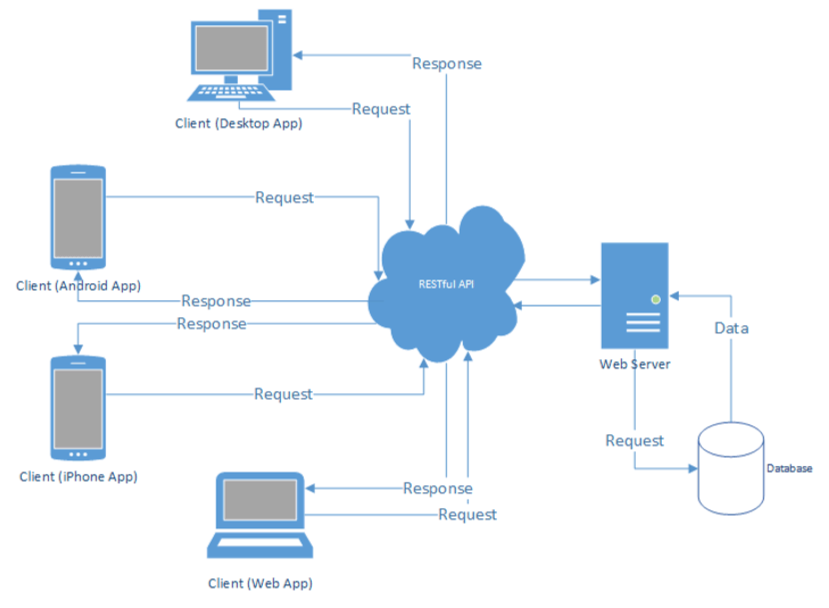
\includegraphics[scale=0.4]{chap1.images/rest-api-flow.png}
              \caption{REST API}
              \label{RESTAPI}
          \end{figure}

\end{itemize}


%__________________________________________________________________________________________________________

\subsection{Environnement matériel}
\noindent Le tableau 1.1 montre les caractéristiques techniques des machines utilisées pour la réalisation de notre application.

\begin{table}[htbp]
    \renewcommand{\arraystretch}{1.5}
    \centering
    \begin{tabular}{|c|c|c|}
        \hline
        Ordinateur             & ASUS TUF F15 & ASUS TUF F15     \\
        \hline
        Propriétaire           & Balti Firas  & Mimouni Med Aziz \\
        \hline
        RAM                    & 32 GO        & 32 GO            \\
        \hline
        Processeur             & i5 11éme     & i5 11éme         \\
        \hline
        Système d’exploitation & Windows 11   & Windows 11       \\
        \hline
    \end{tabular}
    \bigskip
    \caption{Description des machines de développement utilisées}

\end{table}
%____________________________________________________________________________________________

\newpage
\subsection{ Environnement logiciel }

\noindent Les logiciels utilisés pour l’implémentation de notre solution sont les suivants sont les suivants :

\begin{itemize}
    \item[$\bullet$] \textbf{ Figma  :}
          C'est un outil de conception d’interface utilisateur (UI) et d’expérience utilisateur (UX) en ligne. Il permet aux designers de créer des designs d’interface utilisateur . Figma est également utilisé pour collaborer en temps réel. Nous l’avons utilisé dans notre projet pour concevoir les maquettes et les diagrammes de notre application.

          \begin{figure}[ht]
              \centering 
\includegraphics[scale=0.07]{chap1.images/FigmaLogo.png}
              \caption{Figma}
              \label{Figma}
          \end{figure}
          \bigskip


    \item[$\bullet$] \textbf{ Android Studio :}
          C'est un environnement de développement intégré (IDE) développé par Google pour la création d’applications Android. Il est disponible gratuitement pour les développeurs Android. Nous l’avons utilisé dans notre cas pour bénéficier d’un émulateur android servant à débeuguer notre application.

          \begin{figure}[ht]
              \centering 
\includegraphics[scale=0.3]{chap1.images/andoird studio.png}
              \caption{Android Studio}
              \label{Android Studio}
          \end{figure}

          \bigskip

    \item[$\bullet$] \textbf{  Overleaf :}
          C'est un éditeur en ligne de LaTeX, un langage de composition de documents scientifiques et techniques. Il permet aux utilisateurs de créer, de modifier et de collaborer sur des documents LaTeX en temps réel, Tout au long de notre stage de projet de fin d’étude, nous l’avons utilisé pour travailler ensemble sur un seul document et suivre les modifications apportées par chacune de nous en temps réel.

          \begin{figure}[h]
              \centering 
\includegraphics[scale=0.14]{chap1.images/overleaflogo.png}
              \caption{Overleaf}
              \label{fig: Overleaf}
          \end{figure}


          \newpage
    \item[$\bullet$] \textbf{  Spyder :}
          C'est un environnement de développement interactif (IDE) spécialement conçu pour Python, offrant une interface conviviale et des fonctionnalités avancées telles que l'édition de code, l'exploration de variables et la gestion de projets. Nous avons choisi d'utiliser Spyder dans notre cas pour sa simplicité d'utilisation et sa compatibilité avec Python, ce qui nous a permis de développer et de déboguer efficacement notre code .


          \begin{figure}[H]
              \centering
\includegraphics[scale=0.3]{chap1.images/spyder_logo.png}
              \caption{Spyder}
              \label{Spyder}
          \end{figure}



    \item[$\bullet$] \textbf{  Jira :}
          C'est un outil de gestion de projet, conçu pour aider les équipes à planifier, suivre et gérer leurs tâches et leurs projets. Il offre une interface conviviale pour la création de backlogs, l'attribution de tâches, le suivi des progrès et la gestion des délais. Grâce à ses fonctionnalités de collaboration , Jira permet aux équipes de travailler de manière coordonnée et de respecter les délais de manière transparent.

          \begin{figure}[H]
              \centering
\includegraphics[scale=0.2]{chap1.images/jira-logo.png}
              \caption{Jira}

          \end{figure}



    \item[$\bullet$] \textbf{  Slack :}
          C'est une plateforme de communication collaborative propriétaire (SaaS). Nous avons utilisé Slack lors de notre période de stage pour assurer et faciliter la communication avec l’équipe de l’entreprise d’acceuil.

          \begin{figure}[ht]
              \centering
\includegraphics[scale=0.22]{chap1.images/Slack.logo.png}
              \caption{Slack}

          \end{figure}

    \item[$\bullet$] \textbf{ Visme :}
          C'une plateforme de création visuelle en ligne,  nous avons utilisé cette outil pour la création de nos burndown charts.

          \begin{figure}[ht]
              \centering
\includegraphics[scale=0.27]{chap1.images/vismelogo.jpg}
              \caption{Visme}
          \end{figure}

          \newpage
    \item[$\bullet$] \textbf{  Material UI :}
          C'est une bibliothèque de composants React qui facilite la création d'interfaces utilisateurs avec des éléments préconçus basés sur les principes du Material Design de Google. Elle permet une personnalisation poussée et un développement rapide.
          \bigskip
          \begin{figure}[ht]
              \centering
\includegraphics[width=0.13\textwidth,height=1.6cm]{chap1.images/material-ui-logo.png}
              \caption{Material UI}

          \end{figure}
          \bigskip

    \item[$\bullet$] \textbf{ Postman :}
          C'est un outil qui simplifie le test et le développement d'API en permettant d'envoyer des requêtes HTTP et d'analyser les réponses via une interface utilisateur conviviale.

          \begin{figure}[H]
              \centering
\includegraphics[scale=0.28]{chap1.images/Postman-Logo.jpg}
              \caption{Postman}

          \end{figure}
          \bigskip

    \item[$\bullet$] \textbf{ Instagantt  :}
          C'est un outil en ligne intuitif pour la gestion de projets qui permet de créer des diagrammes de Gantt de manière simple et visuelle.
          \bigskip
          \begin{figure}[H]
              \centering
\includegraphics[scale=0.28]{chap1.images/instagantt_logo.jpg}
              \caption{Instagantt }

          \end{figure}
          \bigskip
    \item[$\bullet$] \textbf{ Adobe Photoshop :}
          Nous avons utilisé Photoshop pour la création du logo de notre application. Cet outil nous a permis de concevoir un logo professionnel et attrayant, reflétant l'identité visuelle de notre projet.

          \begin{figure}[H]
              \centering
\includegraphics[scale=0.16]{chap1.images/adobe-photoshop-logo.png}
              \caption{Adobe Photoshop}

          \end{figure}

\end{itemize}



\newpage
\section{Architecture du Système}
\subsection{Architecture logique front-end}

En architecture logicielle, MVVM (Model View ViewModel) est un Design pattern (Modèle de conception) visant à séparer la logique de présentation d’une application en 3 couches :\\

\begin{figure}[ht]
    \centering
    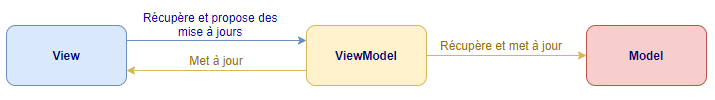
\includegraphics[width=1\textwidth,height=2.3cm]{chap1.images/mvvm.png}
    \caption{Model–view–viewmodel}
\end{figure}


\begin{itemize}
    \item[$\bullet$] \textbf{Model (Modèle) :}
          Le modèle représente la logique métier de l'application et contient les données provenant de bases de données ou d'API externes, optimisées pour la persistance ou la transmission. Il est indépendant de l'interface utilisateur et ne prend pas en compte la manière dont les données seront affichées.
    \item[$\bullet$] \textbf{View (Vue) :}
          La vue est ce que l'utilisateur voit à l'écran. Elle décrit l'interface graphique et fait le lien entre les actions de l'utilisateur et le modèle de vue, définissant l'agencement des composants graphiques et gérant les liaisons de données connectant ces composants aux données du modèle de vue.
    \item[$\bullet$] \textbf{ViewModel (Modèle de Vue) :}
          Le modèle de vue agit comme un médiateur entre le modèle et la vue. Il transforme les données du modèle en formats facilement affichables et manipulables par la vue, permettant à la vue de s'adapter indépendamment des modifications apportées aux données métier et au modèle.


\end{itemize}

\subsection{Architecture physqique}

La figure 1.26 montre l'architecture physique de l'application, incluant les technologies pour le développement web et mobile, et leur connexion à une base de données MySQL.\\

\begin{figure}[ht]
    \centering
    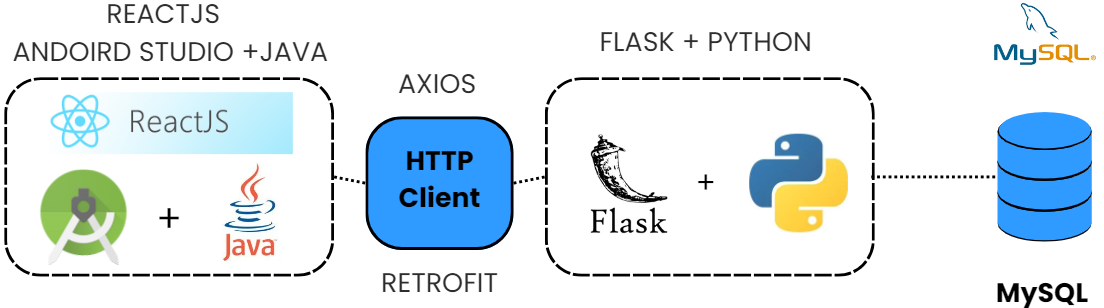
\includegraphics[width=1\textwidth,height=4.6cm]{chap1.images/arch physique.png}
    \caption{Architecture physqique}
\end{figure}
\newpage
\textbf{Fonctionnement:}\\
1- L'utilisateur interagit avec l'interface utilisateur web développée avec ReactJS ou l'application mobile Android.\\
2- Les actions de l'utilisateur déclenchent des requêtes HTTP envoyées via Axios pour le web ou Retrofit pour le mobile.\\
3- Les requêtes sont reçues par le backend Flask, qui traite les demandes en exécutant du code Python.\\
4- Le backend Flask interagit avec la base de données MySQL pour récupérer ou stocker des données.\\
5- Les réponses sont renvoyées au client HTTP, qui les transmet à l'interface utilisateur pour mise à jour.\\

Cette architecture permet une séparation claire des responsabilités entre le frontend et le backend, assurant ainsi une meilleure maintenabilité et évolutivité de l'application.\\
%_________________________________________________________________________________________________________
%____________________________________________________________________________________________________________



\section{Organisation du travail}

Pour assurer une organisation optimale tout au long du développement de notre projet, nous avons mis en place une série de processus et de pratiques collaboratives. Nous avons débuté par des séances de brainstorming, où nous avons généré et partagé des idées. Ces propositions ont ensuite été soumises à des réunions quotidiennes avec notre encadrant professionnel pour validation et conseils. En parallèle, nous avons consulté notre encadrant académique pour le filtrage et le développement des idées. Une fois la phase de conception achevée, nous avons entamé la création du backlog sur Jira, ce qui nous a permis de planifier et d'organiser efficacement les différentes tâches à réaliser. Ensuite, nous avons progressé vers la phase de codage.\\

\begin{figure}[ht]
    \centering
    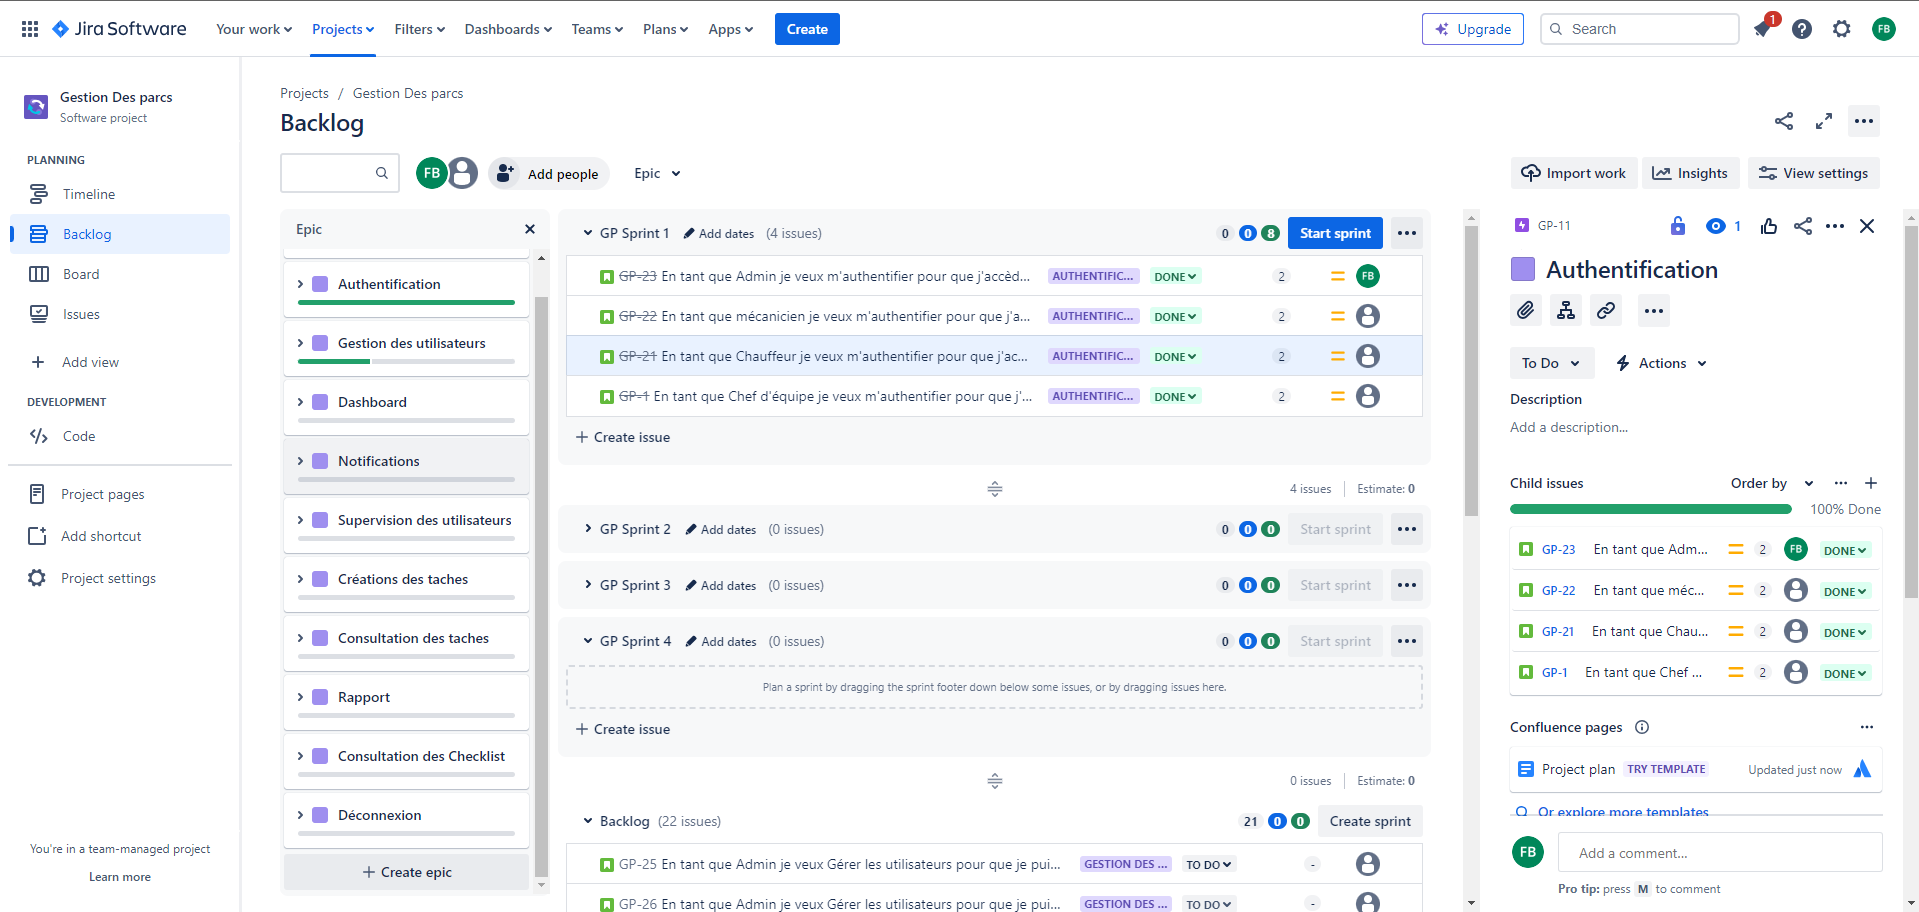
\includegraphics[width=0.9\textwidth]{chap1.images/jira.png}
    \caption{Création du backlog avec Jira}
\end{figure}
\newpage
Pour faciliter la collaboration et le partage du code en temps réel, nous avons opté pour l'utilisation de GitHub. Chacun de nous a pu "pusher" ses changements une fois les tâches accomplies, ce qui nous a permis de suivre l'avancement de chacun et de garantir le respect des délais de réalisation de nos sprints. \\
\begin{figure}[ht]
    \centering
    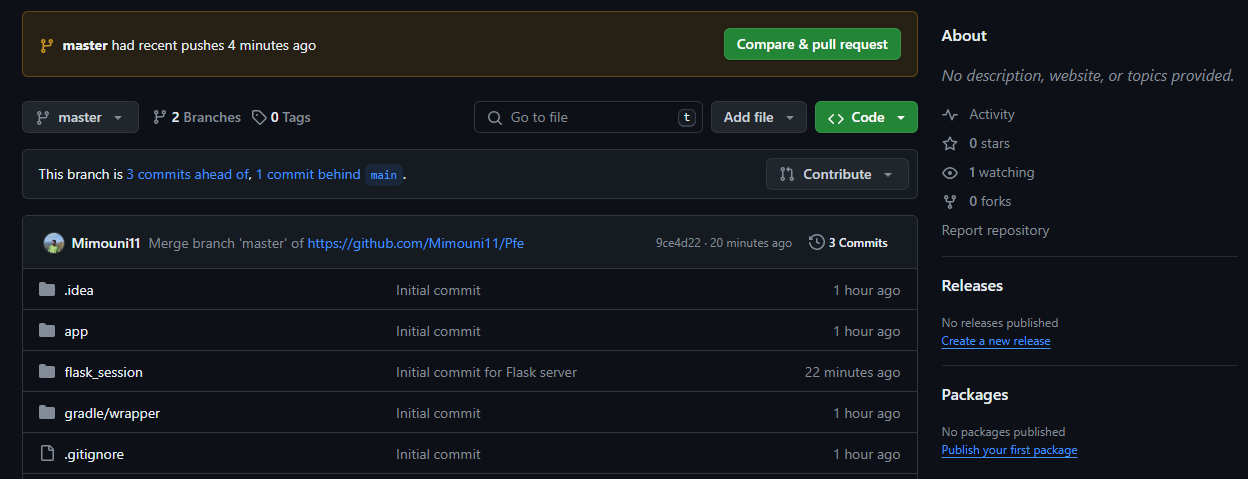
\includegraphics[width=0.9\textwidth]{chap1.images/depot git.png}

    \caption{Dépôt GitHub}
\end{figure}


%_____________________________________________________________________________________________________


\section*{Conclusion}
\addcontentsline{toc}{section}{Conclusion}
\bigskip
\begin{sloppypar}
    Dans ce chapitre, nous avons introduit l’organisme d’accueil, clarifié le cadre du projet  et décrit les choix méthodologiques ainsi que l’architecture. Le prochain chapitre se concentrera sur la planification du projet et la définition des fonctionnalités de l’application.
\end{sloppypar}








